\section{Recovering the calibrator}

In a real life, when a WR network operates for a few years, the WR Device selected
to be a calibrator might become broken. The lack of a WR Calibrator makes it
impossible to connect new devices without recalibrating the whole WR network.
This section presents a method for obtaining the $\Delta_{TX}$, $\Delta_{RX}$
delays for a WR Device so that it can be used as the new WR Calibrator for an
already-deployed network.

\begin{figure}[ht]
	\begin{center}
	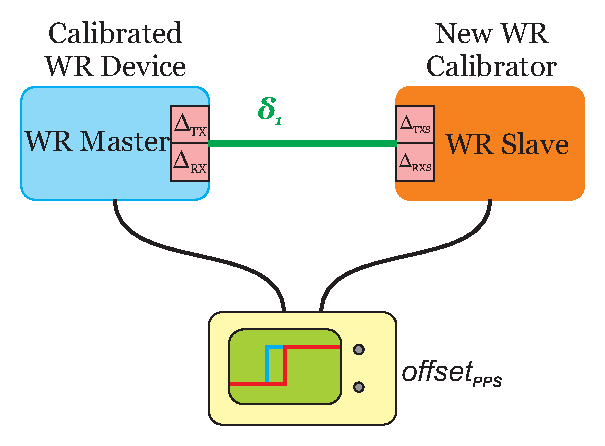
\includegraphics[width=.5\textwidth]{../../figures/calibration/recover_calibrator.ps}
	\caption{Calibrating a new WR Calibrator for an already-existing WR network}
	\label{fig:recover_calibrator}
	\end{center}
\end{figure}

\begin{enumerate}
	\item Initially please set the transmission and reception delays
		($\Delta_{TXS}$, $\Delta_{RXS}$) of the new WR Calibrator to 0, but $\alpha$ has
		to be set to the correct value for fiber $f_1$.
	\item Connect your new WR Calibrator to one of the WR Devices originally
		calibrated to the primary WR Calibrator
		(fig.\ref{fig:recover_calibrator}). Use a short (few meters) fiber of known
		latency and $\alpha$ coefficient or measure it first according to the
		instructions in sections \ref{subsec:refiber} and \ref{subsec:fiasym}. Set
		the WR Calibrator to Slave, and the WR Device to Master mode.
	\item Run the monitoring software on the Slave node (\emph{wr\_mon} for the WR
		Switch or \emph{gui} for the WR PTP Core). Write down the round-trip
		delay and fixed delays of both Master and Slave. The transmission delay of
		the Slave ($\Delta_{TXS}$) should be 0, but its reception delay
		($\Delta_{RXS}$) will be equal to the RX bitslide value $\epsilon_S$. The
		reception delay of the Master ($\Delta_{RXM}$) already includes the bitslide
		value for this device.
	\item Calculate the average (coarse) transmission and reception delay for the
		new Calibrator using the values read from the monitoring software and the
		latency of the fiber ($\delta_1$):
	\begin{equation}
		\Delta'_{TXS} = \Delta'_{RXS} = \frac{1}{2}\Delta_S = \frac{1}{2}(delay_{MM} - \Delta_{TXM} - \Delta_{RXM} - \Delta_{RXS} - \delta_1)
	\end{equation}
	\item Write the $\Delta_{TXS}$ and $\Delta_{RXS}$ delays to the configuration
		of the new WR Calibrator, restart the device, and let it synchronize again
		with the new values.
	\item Measure the Slave to Master offset by comparing 1-PPS signals with an
    oscilloscope. The 1-PPS skew ($skew_{PPS}$) is used as
    a correction value for the coarse transmission/reception delays:
	\begin{align}
		\Delta_{TXS} = \frac{1}{2}\Delta_S - skew_{PPS}\\
		\Delta_{RXS} = \frac{1}{2}\Delta_S + skew_{PPS}
	\end{align}
	\item Update the configuration of the new WR Calibrator to replace the coarse
		delays with $\Delta_{TXS}$, $\Delta_{RXS}$.
	\item The new WR Calibrator can be used to calibrate any other WR Device that is
		supposed to be connected to the existing WR network.\\[12pt]
	{\bf Note:} Please be aware that the measurement errors accumulate. It might
	become an issue if the new calibrator uses values recovered with a WR Device
	that was already calibrated to a recovered calibrator. The longer this chain
	is, the more inaccuracy you should expect from the calibration procedure. To
	minimize this effect, it's better to recover the values for the new WR
	Calibrator using only devices that were calibrated to the primary WR
	Calibrator for a given network.
\end{enumerate}
